\section{Tercer captura: Red local muy chica}
Se realizó una tercer captura en una red local que poseía solamente tres hosts mediante el sniffer implementado por nosotros. La captura duró aproximadamente veinte minutos. En este caso vamos a analizar ambas fuentes de información.
En este experimento se tuvo una red con tres hosts, uno es el router (192.168.1.1), otro es dónde se estaba ejecutando la herramienta de monitoreo (192.168.1.124) mientras que en el equipo restante se estuvo realizando una descarga durante casi todo el tiempo (192.168.1.129).
\subsection{Resultados y análisis}
En el gráfico de barras en el que se compara la información de cada símbolo la fuente S con la entropía de la misma se puede ver que, al igual que en los demás experimentos hubo muchísimos más paquetes broadcast que unicast, aún así el valor de la entropía está bastante cerca de ser el óptimo, el cual es 0.5 ya que son dos símbolos.

\subsection{Conclusiones}



\begin{figure}[h]
  \begin{subfigure}{.5\textwidth}
    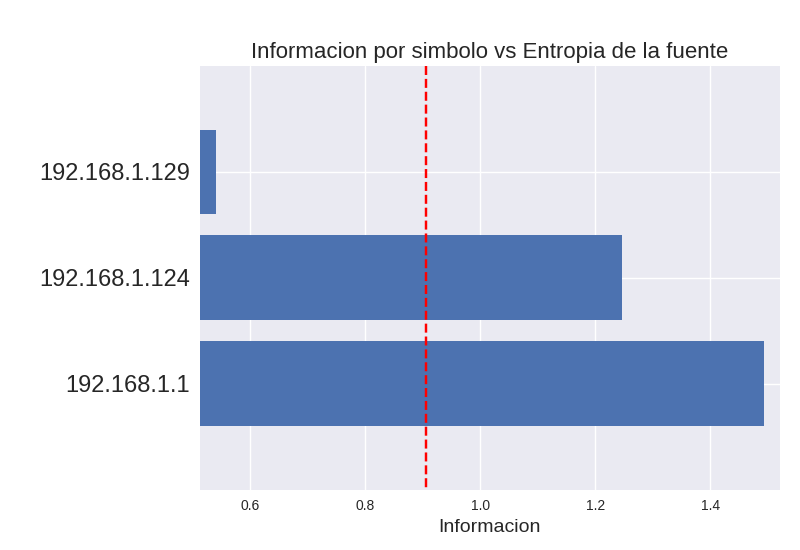
\includegraphics[width=\textwidth]{imagenes/mini_red/mini_red_hosts.png}
  \end{subfigure}
  \label{fig:exp3_hosts_infovsentro}
  \caption{Información de cada símbolo (host) comparada con el valor de la entropía de la fuente de información (red local).}
\end{figure}


\begin{figure}[h]
  \begin{subfigure}{.5\textwidth}
    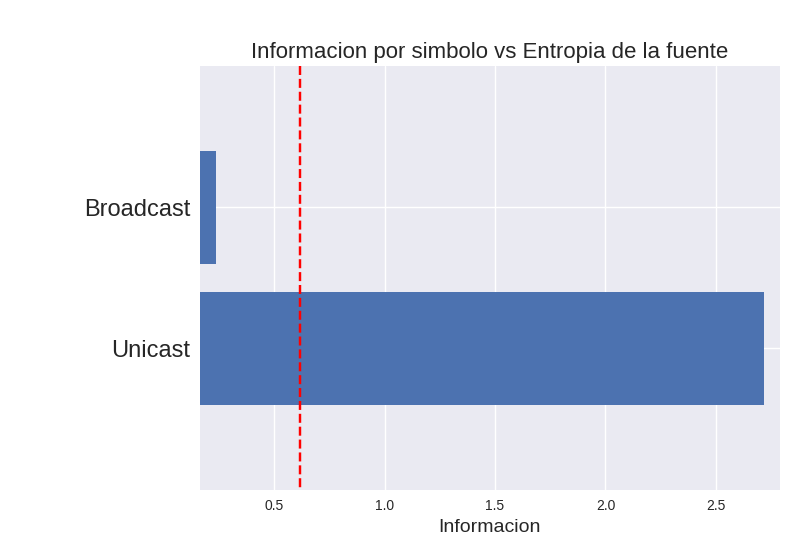
\includegraphics[width=\textwidth]{imagenes/mini_red/mini_red_unicastvsbroadcast.png}
  \end{subfigure}
  \label{fig:exp3_univsbr_infovsentro}
  \caption{Información de cada símbolo (Broadcast / Unicast) comparada con el valor de la entropía de la fuente de información (red local).}
\end{figure}


\section{Cuarta captura: red intermedia}
En este último experimento ejecutamos nuestro sniffer en una casa de comidas rápidas muy concurrida. La red es más grande que una hogareña pero más pequeña que la presentada en el primer experimento. La captura duró aproximadamente media hora.

\subsection{Resultados y análisis}
Como esta red posee muchísimos nodos decidimos realizar el gráfico con los que tienen menor información, en el mismo se pueden ver que hay algunos hosts con menos información que la entropía, mientras que hay otros que no, pero en realidad todo los hosts restantes, es decir los que no fueron incluidos en el gráfico, tienen una información mayor. El host de la ip terminada en 110 es la puerta de enlace predeterminada, lo cual es lógico que tenga mucha interacción con otros hosts. En la red hubo en total 127 hosts. Mientras, en el gráfico de barras en el que se compara la información de los paquetes broadcast contra la de los paquetes unicast se puede ver que hubo una gran diferencia a favor de la cantidad de paquetes broadcast en cuanto a paquetes enviados. Esto es súmamente razonable ya que la gran mayoría de los dispositivos conectados a la red son clientes.

\begin{figure}[h]
  \begin{subfigure}{.5\textwidth}
    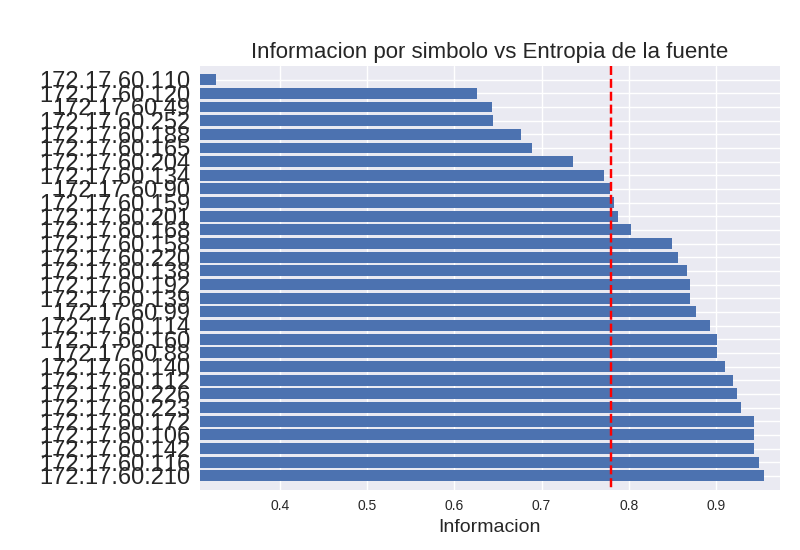
\includegraphics[width=\textwidth]{imagenes/mc/mchosts.png}
  \end{subfigure}
  \label{fig:exp4_hosts_infovsentro}
  \caption{Información de cada símbolo (host) comparada con el valor de la entropía de la fuente de información (red local).}
\end{figure}


\begin{figure}[h]
  \begin{subfigure}{.5\textwidth}
    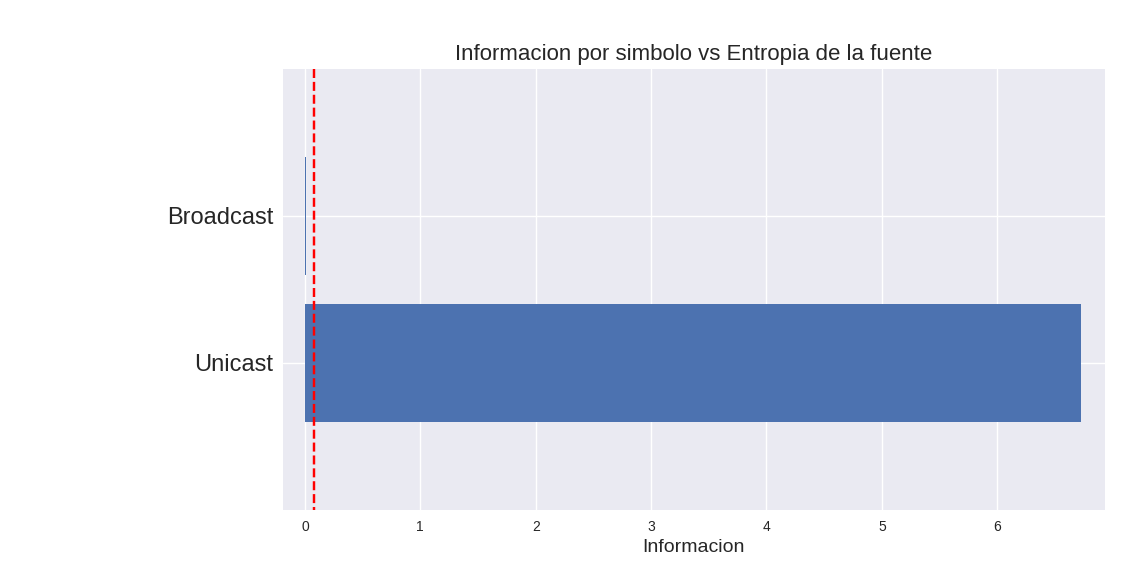
\includegraphics[width=\textwidth]{imagenes/mc/mcbrvsuni.png}
  \end{subfigure}
  \label{fig:exp4_univsbr_infovsentro}
  \caption{Información de cada símbolo (Broadcast / Unicast) comparada con el valor de la entropía de la fuente de información (red local).}
\end{figure}

\begin{figure}[h]
  \begin{subfigure}{.5\textwidth}
    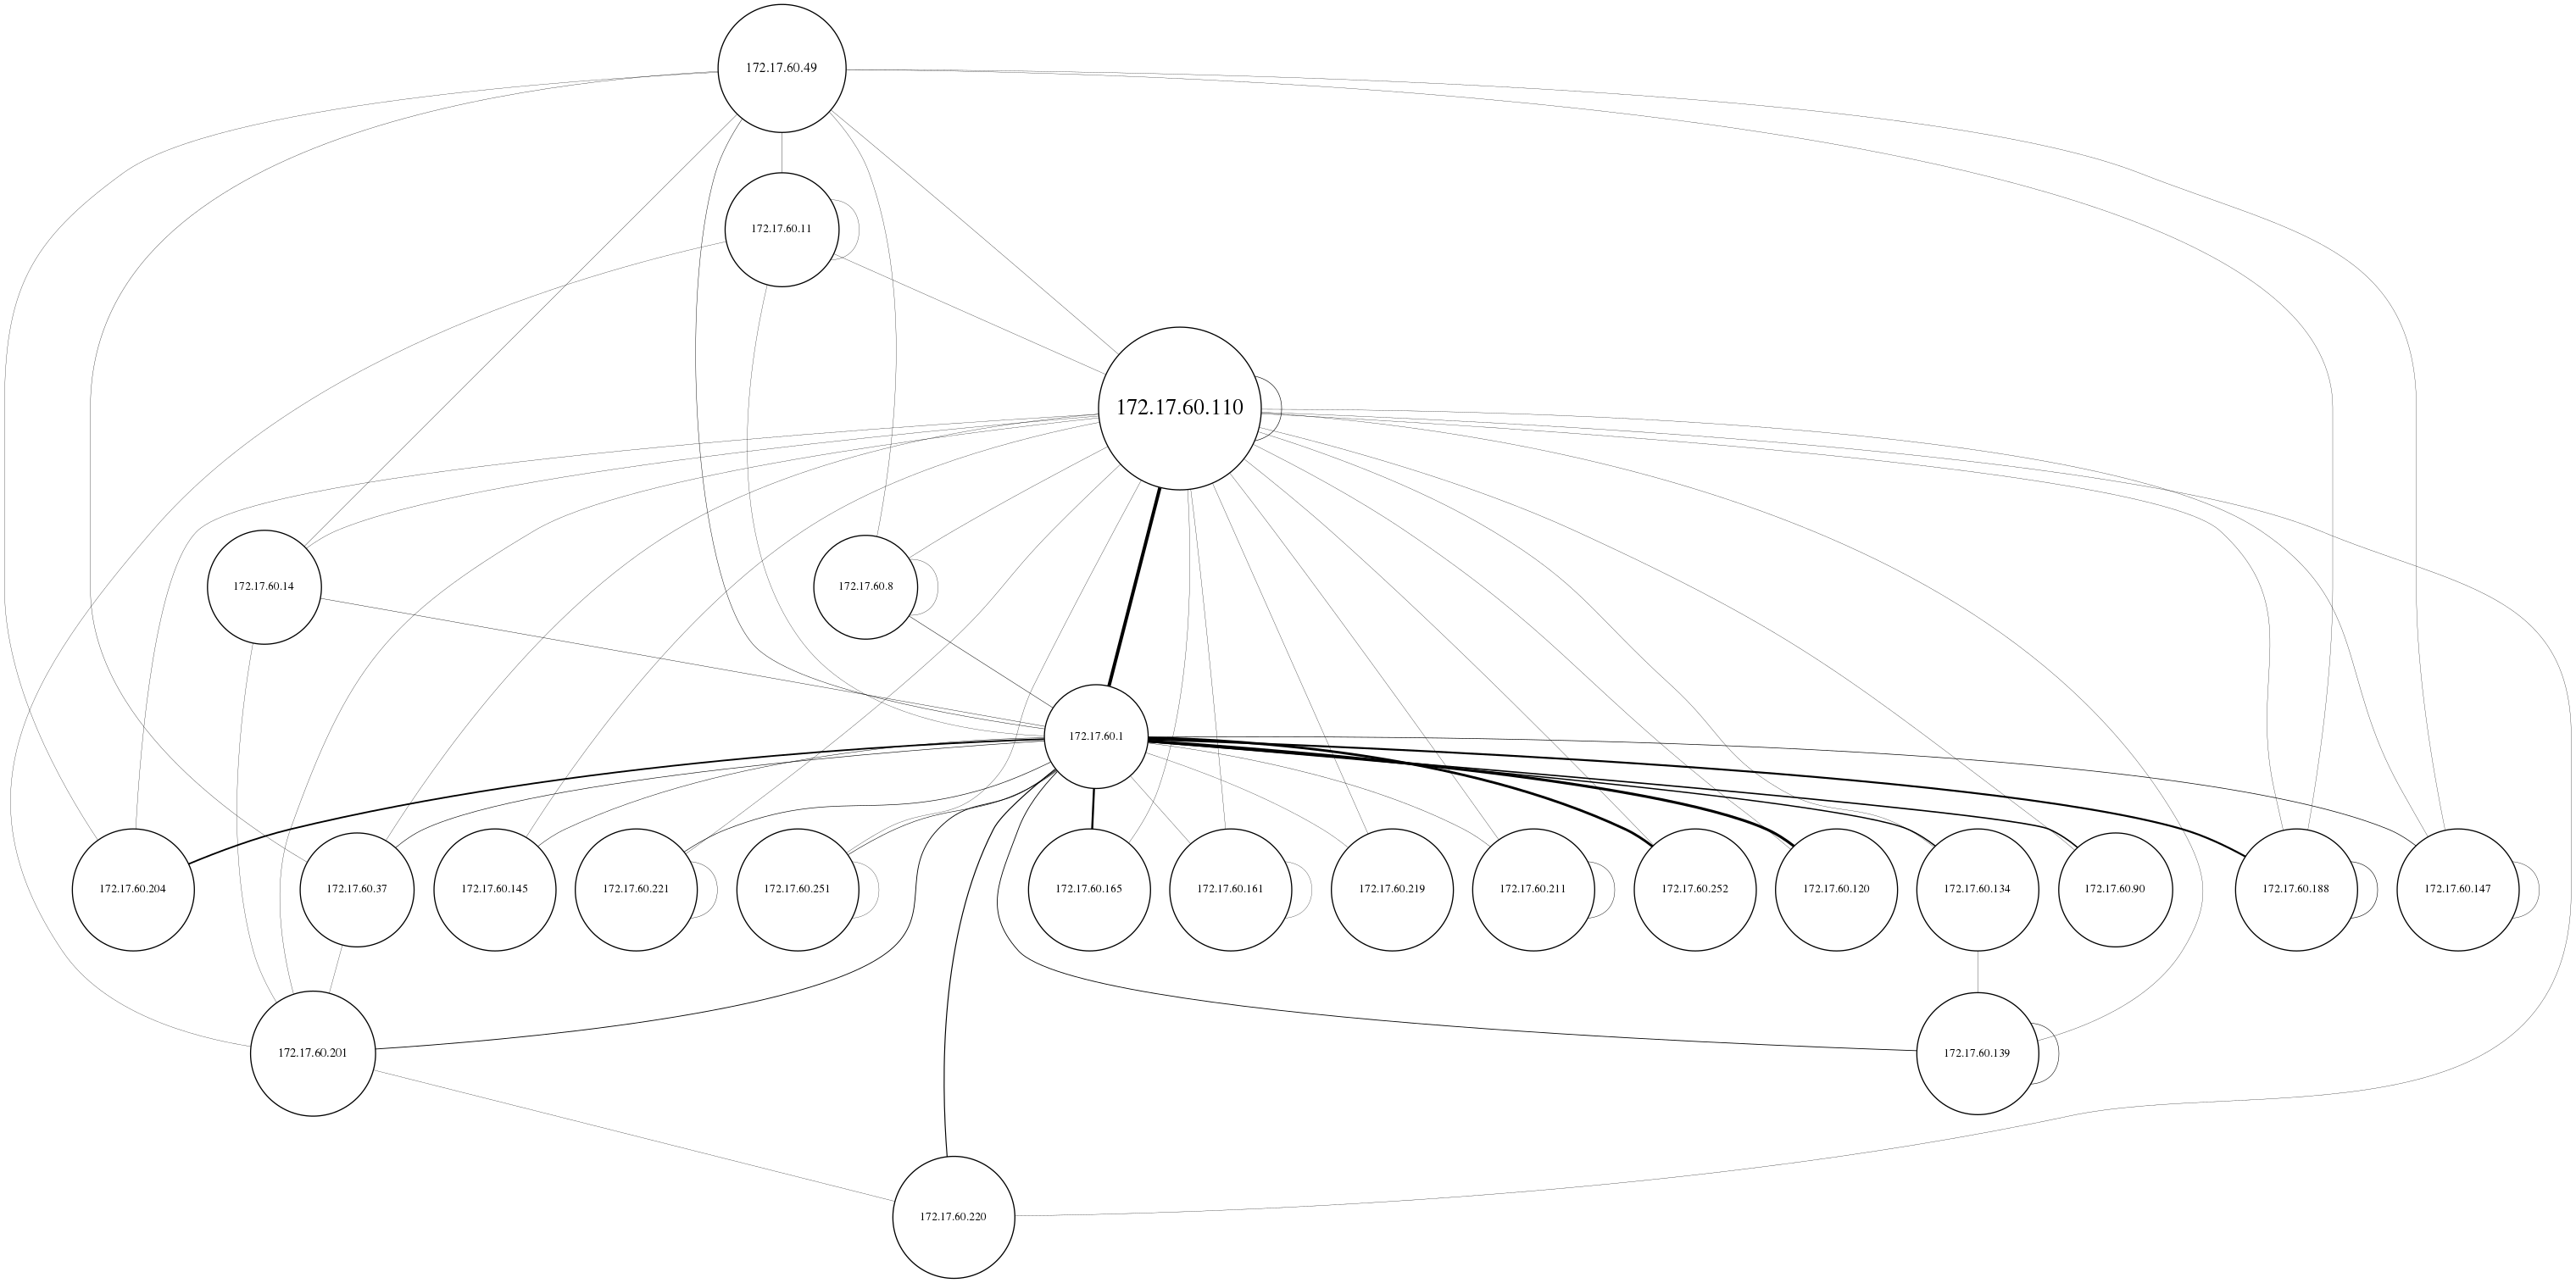
\includegraphics[width=\textwidth]{imagenes/mc/mcRed.png}
  \end{subfigure}
  \label{fig:exp1_labo_red}
  \caption{Diagrama de cómo creemos que está organizada la red de la cuarta captura.}
\end{figure}


\subsection{Conclusiones}


